\documentclass[8 pt]{beamer}
\usepackage[utf8]{inputenc}
\usepackage{amsmath}
\usepackage{multirow}
\usepackage{cancel}
\usepackage{multicol}
\usepackage[document]{ragged2e}
\usepackage{hyperref}
\usepackage{xcolor}
\usepackage{color}
\definecolor{mygray}{gray}{0.7}

\usetheme{EastLansing}
%\usetheme{Pittsburgh}
%\usetheme[height=30pt]{Rochester}
%\usecolortheme{lily}
%\usecolortheme{spruce}

\newcommand{\backupbegin}{
   \newcounter{finalframe}
   \setcounter{finalframe}{\value{framenumber}}
}
\newcommand{\backupend}{
   \setcounter{framenumber}{\value{finalframe}}
}

% -- East Lansing --
\definecolor{mydarkgreen}{RGB}{0,81,40}
\definecolor{mymediumgreen}{RGB}{153, 193, 173}
\definecolor{mylightgreen}{RGB}{229, 239, 234}
\definecolor{mycolor}{RGB}{0,81,40}

\setbeamertemplate{blocks}[rounded][shadow=false]
\setbeamercolor{structure}{fg=mydarkgreen}
\setbeamercolor*{block title}{fg=mydarkgreen, bg=mymediumgreen}
\setbeamercolor*{block body}{fg=black, bg=mylightgreen}

% -- Pittsburgh
%\definecolor{mycolor}{RGB}{51,51,180} %Dark blue
%\definecolor{mycolor}{RGB}{192,57,43} %Dark red
%\definecolor{mycolor}{RGB}{0,81,40} %Dark green

%\setbeamercolor*{title}{use=structure,fg=mycolor,bg=mycolor!12}
%\setbeamertemplate{title page}[default][colsep=-4bp,rounded=true,shadow=false]

%\setbeamertemplate{frametitle}
%{
%	\begin{center}\color{mycolor}\textbf{\Large\insertframetitle}\end{center} \vspace{-5pt}
%}

%\setbeamercolor{structure}{fg=mycolor}
%\setbeamercolor{itemize item}{fg=black}

\setbeamertemplate{blocks}[rounded][shadow=false]
\setbeamercolor*{block title}{fg=mycolor, bg=mycolor!12}
\setbeamercolor*{block body}{fg=black, bg=mycolor!12}

\setbeamercolor*{block title example}{fg=mycolor, bg=mycolor!4}
\setbeamercolor*{block body example}{fg=mycolor, bg=mycolor!12}
\setbeamersize{text margin left=6mm,text margin right=6mm} 
  
%\addtobeamertemplate{navigation symbols}{}{%
%    \usebeamerfont{footline}%
%   \usebeamercolor[fg]{footline}%
%   \hspace{1em}%
%    \insertframenumber/\inserttotalframenumber
%}

\title{Statistical approach to muography}
\date{July 17th 2020}
\author{C\'{e}dric Prie\"els}

 \begin{document}


\begin{frame}
\vspace{-15pt} 
\title{Statistical approach to muography as a non-destructive \\ testing technique for industry problem solving}
\author{C\'{e}dric Prie\"els \\ \vspace{10pt} \textbf{Director} - Pablo Mart\'inez Ru\'iz del \'Arbol \newline \textbf{Co-director} - Carlos D\'iez \\ \vspace{20pt} 
\includegraphics[width= 0.15\textwidth]{figs/image_UC.png} \hspace{10pt} 
\includegraphics[width= 0.16\textwidth]{figs/muonSystems.png} \newline \vspace{20pt} Universidad de Cantabria \newline Muons systems \newline  \begin{center} \large{\textbf{July 17th 2020}} \end{center}}

\date{}
\vspace{15pt}
\maketitle

\centering
  
\end{frame}


\begin{frame}{Outline}

	\begin{itemize}
		\item Introduction \vfill
		\item Muons and muography \vfill
		\item Statistical basis of the algorithm
		\begin{itemize}
			\item Probability density functions
			\item Kernel density estimation
			\item Monte-Carlo simulations
			\item Likelihood minimization
		\end{itemize} \vfill
		\item The algorithm \vfill
		\item Results obtained \vfill
		\item Conclusions \vfill
	\end{itemize}

\end{frame}






%Introduction
\begin{frame}{}
	\centering
	\huge{\textbf{\color{mycolor} Section I}} \newline
	\LARGE{\textbf{\color{mycolor} General introduction \color{black}}} \vfill
	
	\LARGE{\textbf{\color{black} Main goal of this work \color{black}}}\newline \vspace{10pt} Develop a new framework allowing to perform a muography experiment to characterize the inner properties of physical objects using data science and advanced statistical models. \vfill
\end{frame}















%Theoretical introduction
\begin{frame}{Particle physics and muons}

\begin{minipage}[c]{.54\textwidth}
The Standard Model \textbf{describes the fundamental particles} existing and their interactions:
\begin{itemize}
	\justifying
	\item Introduced in the 1970s and still considered to be valid, but probably incomplete
	\item Simple in concept but extremely precise
	\item Lots of successful predictions made over the years, such as the existence of the top quark and the Higgs boson
\end{itemize}
\end{minipage} \hfill
\begin{minipage}[c]{.42\textwidth}
	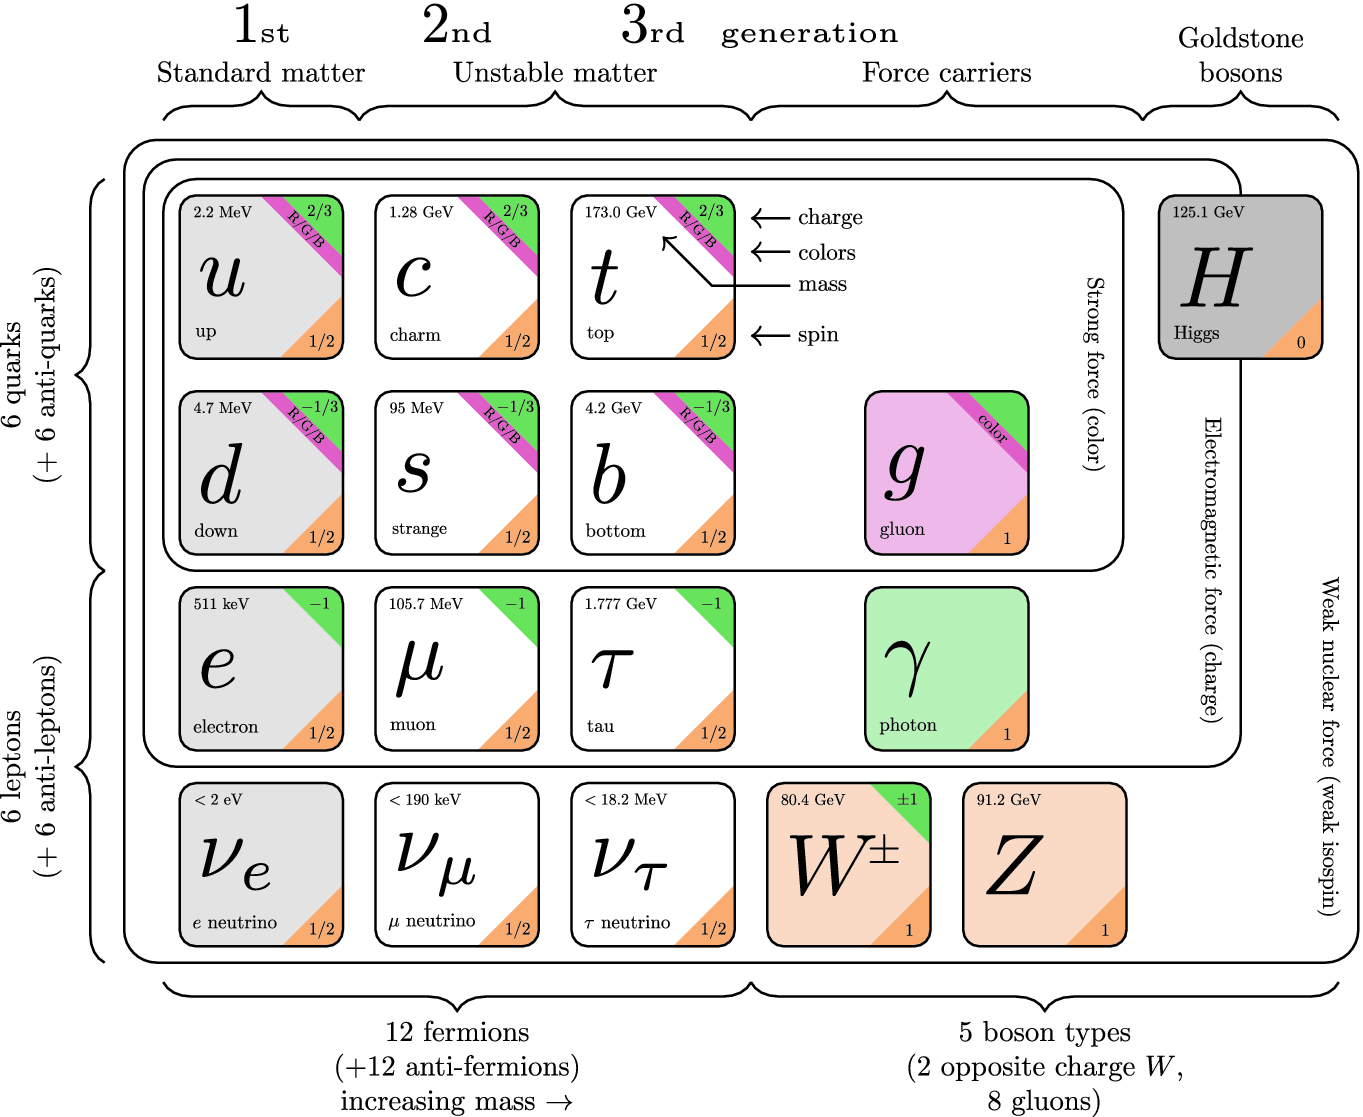
\includegraphics[width=5cm, height=4.2cm]{figs/SMFermions.png}
\end{minipage} \hfill \vfill

\begin{exampleblock}{} Muons \end{exampleblock}
\begin{itemize}
	\justifying
	\item Muons $\mu^-$ are one of the 12 fundamental particles existing
	\item They have a relatively small interaction cross-section with ordinary matter, allowing them to cross material without being stopped, making them interesting.
\end{itemize} \vfill
\end{frame}


\begin{frame}{Cosmic rays}
\justifying
Comic rays are a \textbf{constant flux of high energy particles} reaching the Earth:
\begin{itemize}
	\justifying
	\item Mostly made out of protons and atomic nuclei
	\item Trigger a decay chain by interacting with the atmosphere, producing muons
	\item Muons are not stable ($\tau \simeq 2.2\mu$s) but relativity can make them live long enough to reach the ground $\rightarrow$ 10.000 cosmic muons are observed per $m^2$ and per minute at sea level.
\end{itemize} \vfill

\begin{minipage}[c]{.98\textwidth}
	\begin{center}
	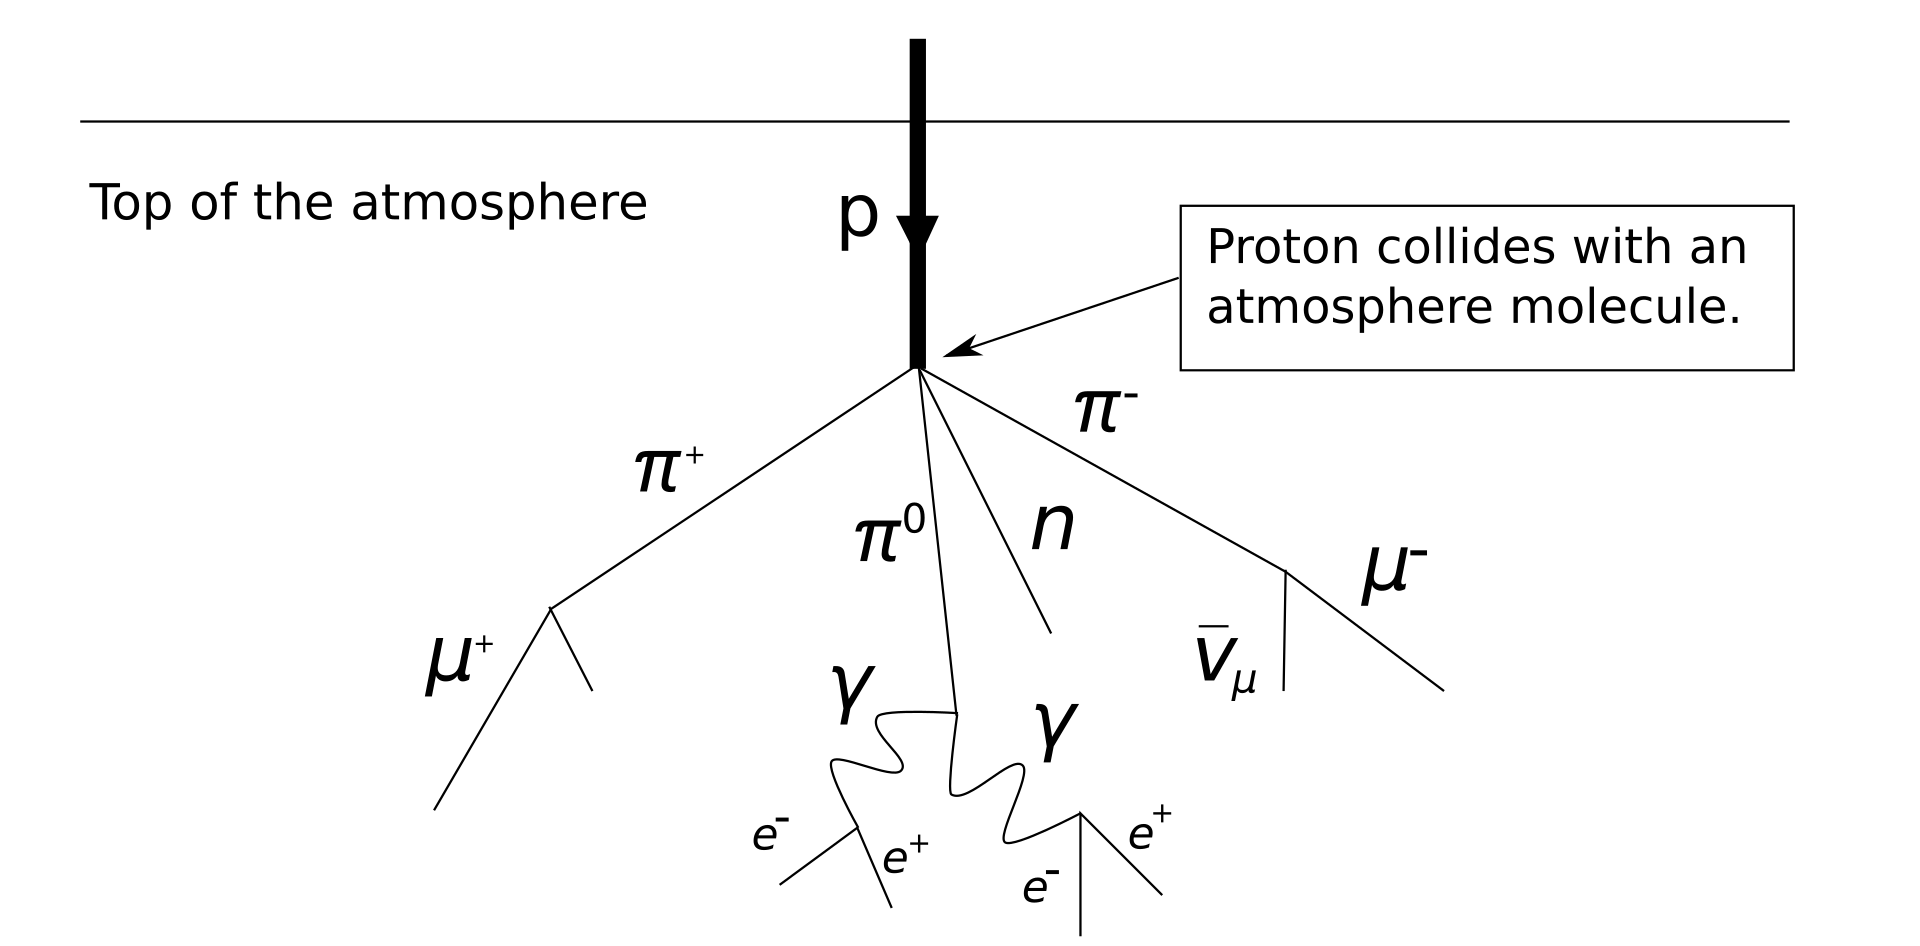
\includegraphics[width=8cm, height=4cm]{figs/cosmic.png}
	\end{center}
\end{minipage} \hfill \vfill
\end{frame}

\begin{frame}{Interaction with matter}

\end{frame}

\begin{frame}{Muon tomography}

\end{frame}

\begin{frame}{Experimental setup}

\end{frame}








%Statistical basis
\begin{frame}{Statistical basis}

\end{frame}

\begin{frame}{Probability density functions}

\end{frame}

\begin{frame}{Kernel density estimation}

\end{frame}

\begin{frame}{Monte-Carlo simulations}

\end{frame}

\begin{frame}{Maximum likelihood estimation}

\end{frame}








%The algorithm
\begin{frame}{General idea}

\end{frame}

\begin{frame}{MuonState}

\end{frame}

\begin{frame}{Surfaces and Volumes}

\end{frame}

\begin{frame}{Cylinders and pipes}

\end{frame}

\begin{frame}{Propagator}

\end{frame}

\begin{frame}{Likelihood}

\end{frame}











%Results obtained
\begin{frame}{Generator validation}

\end{frame}

\begin{frame}{Pipes geometries}

\end{frame}

\begin{frame}{Kernel density functions}

\end{frame}

\begin{frame}{Likelihood curves}

\end{frame}








%Conclusions
\begin{frame}{Conclusion}

\end{frame}

\begin{frame}{Future improvements}

\end{frame}










%Back up
\begin{frame}{}
	\centering
	\huge{\textbf{\color{mycolor} Thank you  \color{black}}} \newline
	\LARGE{\textbf{\color{mycolor} for your attention! \color{black}}} \vfill

	Any questions? \vfill
\end{frame}

\appendix
	\backupbegin
	


\backupend


 \end{document}